\section{Introduction}

Gravitational wave observations now provide direct access to the strong-field, dynamical regime of compact-binary coalescence. As detector sensitivities improve and high-signal-to-noise-ratio detections become more likely, the late inspiral, merger, and ringdown will offer increasingly stringent tests of the general-relativistic description of black holes \cite{Abbott2025GWTC3GR,Yunes2025GWTests,Yagi2016_BHTestsGR,Berti2015,Abac2025GW250114}. Recent detections have reached signal-to-noise ratios as high as $80$, enabling tests of Hawking's area law and improved measurements of the remnant black hole \cite{LVK2025GW250114}. These developments motivate numerical studies of how specific beyond-GR effects could appear in the late-inspiral, merger, and ringdown waveform.

For many alternative theories of gravity, analytic approximations are insufficient near merger, while numerical simulations require a well-posed initial-value formulation, stable gauge choices, and controlled constraint behavior as we mentioned in the prior chapter. Considerable effort has been devoted to developing formulations and approximation schemes that permit nonlinear simulations beyond GR \cite{Cardoso2012NRHEP,Corman2024NonlinearModificationsGR,Afshordi2024BlackHolesInsideOut,Bambi2025Mimickers,Bernard2025GenericEFTGWTests}. Examples include studies of dynamical Chern--Simons gravity \cite{Alexander2009,Okounkova2019}, Einstein-dilaton-Gauss-Bonnet theory \cite{Okounkova:2020rqw,Okounkova2020}, modified gauge choices in Einstein-scalar-Gauss-Bonnet theory \cite{Ripley2020a,Ripley2020b}, the ``fixing the equations'' approach \cite{Cayuso2020}, and auxiliary-field formulations for higher-curvature systems, including quadratic gravity \cite{Held2021,Held2023,Held2025,East2023,Taillte2025}. See also Ref.~\cite{Corman2024} for a more detailed comparison of these approaches.

In this chapter, we focus on Einstein--Maxwell--dilaton--axion (EMDA) theory. EMDA extends Einstein--Maxwell theory by coupling the electromagnetic field to a dilaton and an axion, and it arises as a low-energy limit of heterotic string theory \cite{Sen1992,Sen1995}. The theory admits rotating charged black hole solutions, such as the Kerr--Sen spacetime, which differs from Kerr--Newman by the presence of nontrivial dilaton and axion fields. In the last chapter we investigated the stability of black holes and black hole hair in EMDA theory \cite{PopeRohrerWhiting2025,Carroll2026KerrSenStability}, and black hole shadow studies using Event Horizon Telescope observations have not ruled out Kerr--Sen black holes \cite{Sahoo2024PRD,Sahoo2025}. These features make EMDA a useful setting in which to study how additional matter fields can influence compact-binary dynamics and gravitational radiation.

Charged binary black holes have also been studied in Einstein--Maxwell gravity \cite{Bozzola2019,Zilhao2012,Zilhao2014,Bozzola2021,Bozzola2023ExtremalChargedMergers,Luna2022ChargedBBHKicks}. These simulations show that electromagnetic charge can modify the orbital dynamics, emitted radiation, and recoil of the remnant. In one analysis, the GW150914 signal was found to be compatible with charge-to-mass ratios as large as $Q/M\sim0.3$ ~\cite{Bozzola2021}. These studies demonstrate that charge alone can alter the inspiral, merger, radiation content, and remnant properties. In EMDA theory, charge also sources additional scalar and pseudoscalar fields, so charged binaries provide a natural setting in which to study how electromagnetic and beyond-GR matter jointly affect the gravitational waveform.

The goal of this chapter is to take a step toward an exploratory waveform catalog for charged binary black holes within EMDA. We simulate inspiraling charged binary black holes and compare the resulting gravitational waveforms with neutral general relativistic reference waveforms having the same mass ratio and spin. The cases considered here include charge-to-mass ratios much larger than those expected for astrophysical black holes \cite{Gibbons1975VacuumPolarization,Pan2019BlackHoleDischarge}. Our aim is therefore not to construct immediately realistic astrophysical templates, but to identify regimes in which charge and the additional EMDA fields produce appreciable changes in the binary dynamics and gravitational wave signal.

These comparisons should be interpreted as fixed parameter waveform comparisons rather than as a complete parameter-estimation study. Compact-binary waveforms are highly degenerate, and differences between an EMDA waveform and a GR waveform may be partially mimicked by varying intrinsic binary parameters such as the mass ratio, spins, total mass scale, or eccentricity\cite{Hannam2013MassSpinDegeneracy,Vallisneri2013StealthBias}. Moreover, because the comparisons in this chapter are made against neutral GR rather than charged Einstein--Maxwell binaries, the resulting differences should be understood as the combined effect of charge, modified orbital dynamics, and the additional EMDA fields, rather than as isolated dilaton or axion signatures.

The catalog presented here is therefore intended as an initial step toward a more complete study of EMDA binary black hole phenomenology. In particular, it identifies regions of parameter space where charged EMDA binaries produce appreciable waveform differences relative to neutral GR and motivates future comparisons among neutral GR, Einstein--Maxwell, and EMDA binaries.

\section{Einstein--Maxwell--Dilaton--Axion Theory}
\label{sec:emda}

We consider Einstein--Maxwell--dilaton--axion (EMDA) theory, in which the Einstein--Maxwell system is supplemented by a scalar dilaton field $\phi$ and a pseudoscalar axion field $\kappa$. With the conventions used here, the action is
\begin{equation}
\begin{aligned}
S = \int \mathrm{d}^4 x,\sqrt{-g}\Big[
&\frac{R}{8\pi}
-2\nabla_a\phi\nabla^a\phi
-e^{-2\alpha_0\phi}F_{ab}F^{ab} -\frac{1}{2}e^{4\alpha_1\phi}\nabla_a\kappa\nabla^a\kappa
-\kappa F_{ab}({}^{*}F)^{ab}
\Big],
\end{aligned}
\label{eq:emda_action}
\end{equation}
where $R$ is the Ricci scalar, $F_{ab}$ is the $U(1)$ field strength, and $({}^{*}F)_{ab}$ is its dual. The constants $\alpha_0$ and $\alpha_1$ determine the coupling strengths between the electromagnetic field and the dilaton and axion fields.

As we mentioned in the prior chapter different choices of $\alpha_0$ and $\alpha_1$ correspond to different members of this class of theories. The parameter $\alpha_0$ controls the exponential coupling between the dilaton and the electromagnetic field, while $\alpha_1$ controls the exponential coupling of the dilaton to the axion kinetic term. For example, the choice $(\alpha_0,\alpha_1)=(\sqrt{3},0)$ gives the Kaluza--Klein value of the dilaton coupling \cite{Horne1992,Mignemi1993_ChargedStringBH}. In the simulations presented here, we fix
\begin{equation}
(\alpha_0,\alpha_1)=(1,1),
\end{equation}
which corresponds to the coupling values associated with the low-energy limit of heterotic string theory \cite{Sen1992,Sen1995}.

For this choice of couplings, the theory admits rotating charged black hole solutions of the Kerr--Sen type \cite{Sen1992}. These solutions reduce to Kerr in the limit of vanishing electromagnetic charge, but for nonzero charge the black hole is accompanied by a nontrivial dilaton field and, in the rotating case, a nontrivial axion field. The structure of these fields is known analytically for a single isolated black hole; the solution we summarized in the previous chapter.

To simulate inspiraling binary black holes, we construct approximate charged binary black hole initial data and evolve the full EMDA system numerically. This allows us to compare the resulting gravitational waveforms against neutral general relativistic reference waveforms and to identify how the combined electromagnetic, dilaton, and axion fields influence the inspiral and merger.

\section{Numerical Methods}
\label{sec:methods}

To study the strong-field dynamics and gravitational radiation from inspiraling charged black hole binaries in Einstein--Maxwell--dilaton--axion (EMDA) theory, we evolve the full EMDA system as a Cauchy initial-value problem. The spacetime metric is evolved using the BSSN formulation \cite{Shibata1995_BSSN,Baumgarte1999_BSSN,Baumgarte2010}, together with puncture gauge conditions \cite{Campanelli2006,Baker2006}. The electromagnetic, dilaton, and axion fields are evolved using the matter evolution equations obtained from the $3+1$ decomposition of the EMDA equations of motion. The full evolution system is summarized earlier.

The simulations are initialized with approximate charged binary black hole initial data and evolved through the late inspiral, merger, and ringdown. During the evolution, we extract gravitational radiation and monitor the matter fields, constraints, and quasilocal horizon quantities in order to assess the dynamics and numerical consistency of the solutions.

\subsection{Numerical implementation}
\label{sec:code_description}

For the simulations presented here, we evolve the EMDA system using the same code described in Chapter~2, \texttt{Dendro-GR}. Further details on the \texttt{Dendro-GR} infrastructure, including its adaptive wavelet-refinement strategy, code-generation framework, scalability, and previous applications to binary black hole simulations, can be found in the previous chapter and in Refs.~\cite{Fernando2019,Fernando2019b,Fernando2023,Black2025_ORBIT}. In particular, \texttt{Dendro-GR} has been shown to perform well for intermediate-mass-ratio inspiral simulations, where adaptive refinement is especially useful for resolving disparate length scales \cite{Fernando2019b,Black2025_ORBIT}.

As before, throughout each evolution, we monitor the Hamiltonian and momentum constraints, as well as the electromagnetic divergence constraints. These quantities are used to track the consistency of the numerical solution and to assess whether the chosen refinement parameters adequately resolve the relevant dynamics.

We also extract quasilocal horizon quantities using a modified version of the \texttt{BHaHAHA} apparent-horizon finder \cite{Etienne2026BHaHAHA}. In addition to locating the apparent horizons, this modified version computes the horizon mass, spin, and electric charge during the evolution.
\subsection{Controlling the eccentricity}
\label{sec:eccentricity_control}

In this chapter, we focus on approximately quasicircular inspirals. For uncharged binary black holes, post-Newtonian methods can be used to choose initial momenta that reduce the orbital eccentricity.Post Newtonian methods approximate general relativity by expanding the equations of motion in powers of $v/c$, where $v$ is the characteristic orbital speed. They are most accurate when the objects are moving slowly compared with the speed of light and are separated by distances large compared with their gravitational radii. In compact binary systems, post Newtonian theory provides analytic expressions for the orbital dynamics and gravitational waveform during the inspiral, before the late merger regime where full numerical relativity is needed. In the EMDA system, however, the presence of electromagnetic, dilaton, and axion fields complicates the construction of low-eccentricity initial data. Post-Newtonian treatments have been developed for Einstein--Maxwell theory and for several scalar-modified theories of gravity~\cite{Khalil2018_EMD_EOB,Yagi2012_QuadraticGravityPN,Julie2019_EsGB_PN,Gupta2025_EinsteinMaxwell2PN}. Here we adopt a simpler prescription based on the charged-binary argument used in Ref.~\cite{Bozzola2021}.

At Newtonian order, both the gravitational and electromagnetic interactions are central forces. For two charged compact objects, the Coulomb interaction modifies the effective strength of the attractive force. Denoting the charge-to-mass ratio of each black hole by
\begin{equation}
\lambda_i = \frac{Q_i}{M_i},
\end{equation}
the leading-order effect of the electromagnetic interaction can be incorporated through the replacement of Newton's constant
\begin{equation}
G \rightarrow \tilde{G} = G\left(1-\lambda_1\lambda_2\right).
\end{equation}
In units where $G=1$, this becomes
\begin{equation}
\tilde{G} = 1-\lambda_1\lambda_2 .
\end{equation}
Thus, like-signed charges reduce the effective attraction, while oppositely signed charges increase it. We first compute the momenta required for the corresponding uncharged binary to be approximately quasicircular using post-Newtonian estimates, and then rescale the orbital momenta according to the charge-dependent effective coupling. At leading Newtonian order, this corresponds to scaling the tangential momentum by
\begin{equation}
p_t \rightarrow p_t \sqrt{1-\lambda_1\lambda_2}.
\end{equation}
This prescription assumes that the dominant correction to the initial orbital parameters comes from the electromagnetic interaction; possible direct corrections from the dilaton and axion fields are not included in the initial momentum estimate.

We focus on quasicircular orbits because gravitational wave emission tends to circularize isolated compact binaries during the inspiral \cite{Peters1964,Pfeiffer2007ReducingEccentricity}.The initial momenta for the corresponding uncharged binaries are computed using the \texttt{NRPyPN} package~\cite{Etienne2023_NRPyPN}. This package provides post-Newtonian estimates for low-eccentricity binary black hole initial data compatible with Bowen--York/TwoPunctures data~\cite{Healy2017_PNQuasicircular,RamosBuades2019_EccRed}. We then apply the charge-dependent rescaling described above to obtain the momenta used in the charged evolutions.

Although approximate, this prescription yields eccentricities that are adequate for the exploratory comparisons performed here, as illustrated in Figs.~\ref{fig:orbital_dynamics_q1_q2} and~\ref{fig:orbital_dynamics_q4_q8}. This figure demonstrates that the black hole trajectories are approximately circular. 
\FloatBarrier
\begin{figure}[p]
\centering


\subfloat[$q=1$: black hole separation.\label{fig:bh_separation_q1}]{%
    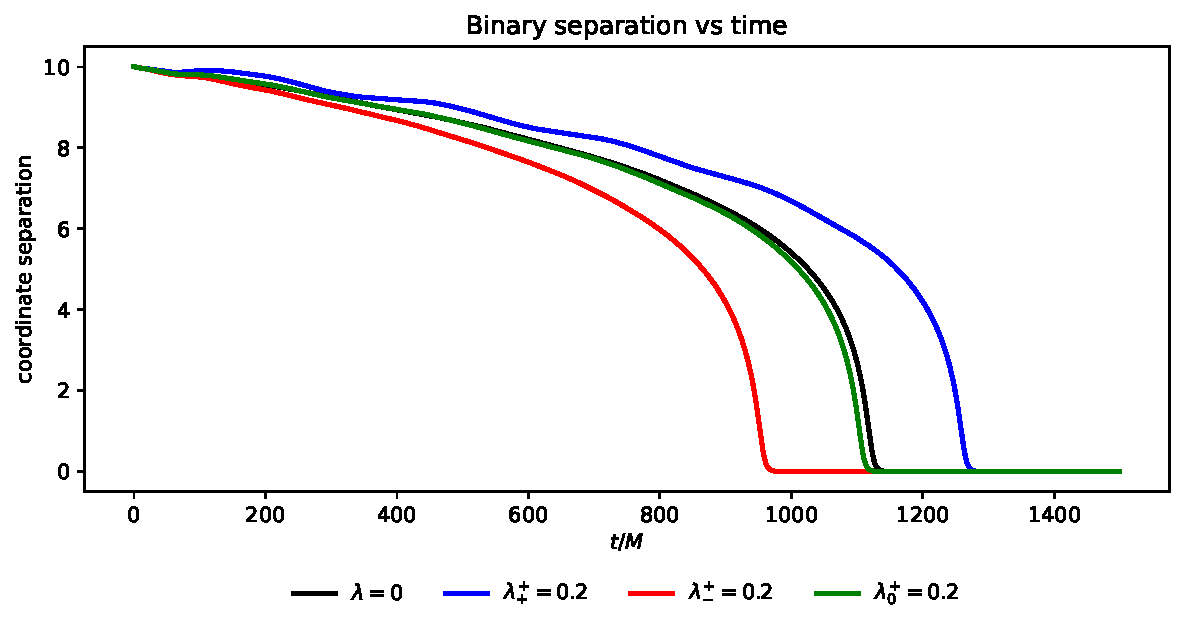
\includegraphics[height=0.22\textheight,keepaspectratio]{Figures/Chapter_2/Q1_SPIN_04_high_charge_separation_comparison.pdf}%
}
\hfill
\subfloat[$q=1$: orbital trajectories.\label{fig:bh_xy_q1}]{%
    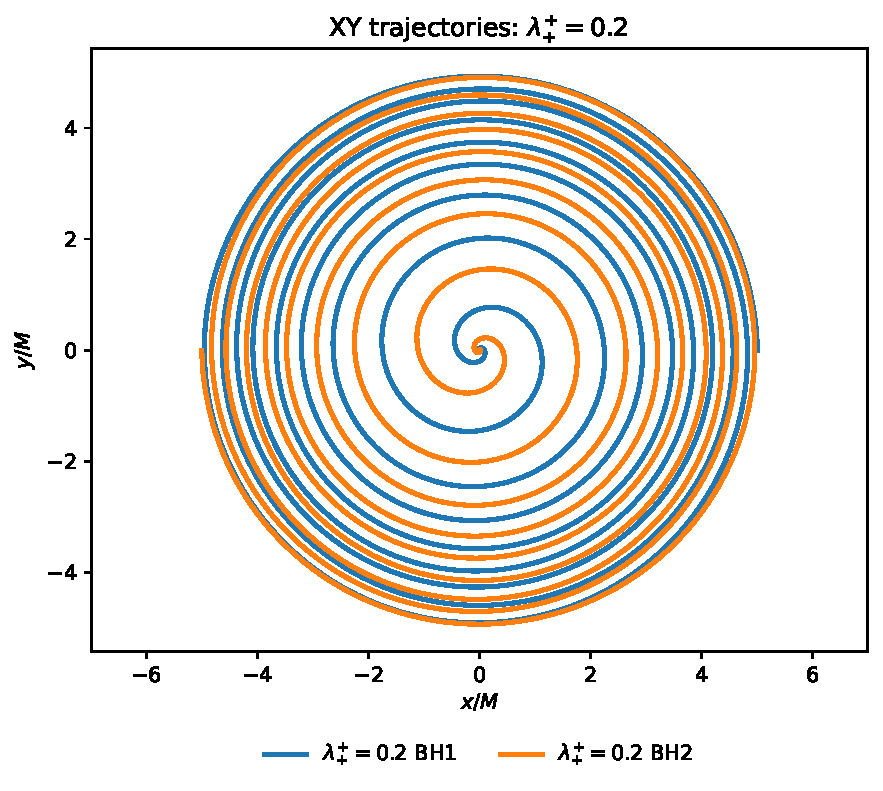
\includegraphics[height=0.22\textheight,keepaspectratio]{Figures/Chapter_2/Q1_SPIN_04_high_charge_Q0p1_pp_xy_trajectory.pdf}%
}

\vspace{1.0em}

\subfloat[$q=2$: black hole separation.\label{fig:bh_separation_q2}]{%
    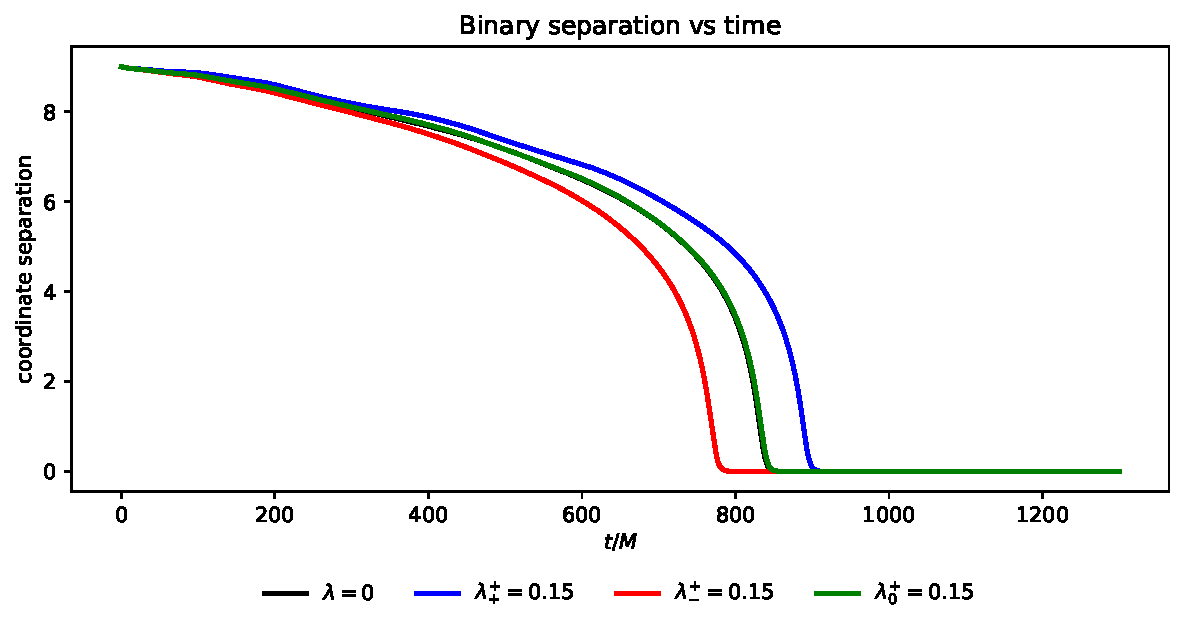
\includegraphics[height=0.22\textheight,keepaspectratio]{Figures/Chapter_2/Q2_SPIN_04_high_charge_separation_comparison.pdf}%
}
\hfill
\subfloat[$q=2$: orbital trajectories.\label{fig:bh_xy_q2}]{%
    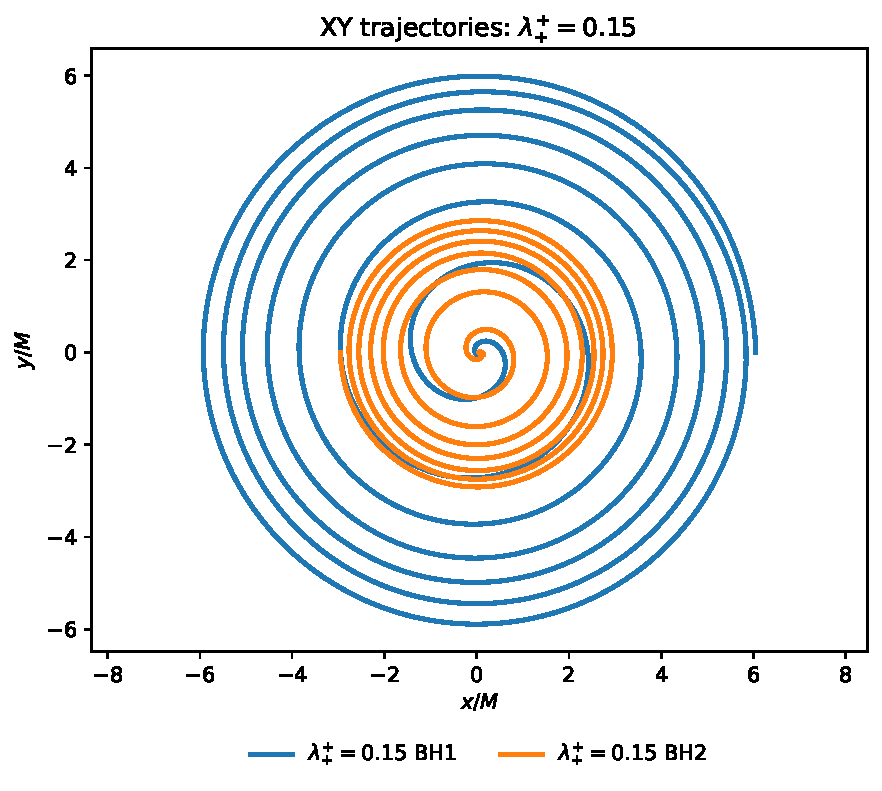
\includegraphics[height=0.22\textheight,keepaspectratio]{Figures/Chapter_2/Q2_SPIN_04_high_charge_Q0p15_pp_xy_trajectory.pdf}%
}

\caption{Orbital dynamics for the $q=1$ and $q=2$ configurations. For each mass ratio, the left panel shows the coordinate separation as a function of time, while the right panel shows representative coordinate trajectories in the orbital plane. The charge configuration affects both the inspiral time and the orbital phasing by modifying the effective interaction between the black holes. The trajectories are approximately quasicircular until the final plunge, which begins once the separation drops below roughly $6M$. Here $\lambda$ denotes the magnitude of the charge-to-mass ratio, $|Q|/M$, assigned to each charged black hole; neutral black holes have $\lambda=0$. The superscript and subscript indicate the charge configuration, with the larger black hole assigned the positive charge in unequal-mass cases. Thus, $\lambda^{+}_{+}$ denotes two positively charged black holes, $\lambda^{+}_{-}$ denotes oppositely charged black holes, and $\lambda^{+}_{0}$ denotes one positively charged and one neutral black hole. The $\lambda=0$ case is the GR reference waveform. In the trajectory plots, orange and blue denote the paths of the heavier and lighter black holes, respectively, with the initial data chosen so that the center of mass is at the origin.}
\label{fig:orbital_dynamics_q1_q2}

\end{figure}
\FloatBarrier
\begin{figure}[p]
\centering


\subfloat[$q=4$: black hole separation.\label{fig:bh_separation_q4}]{%
    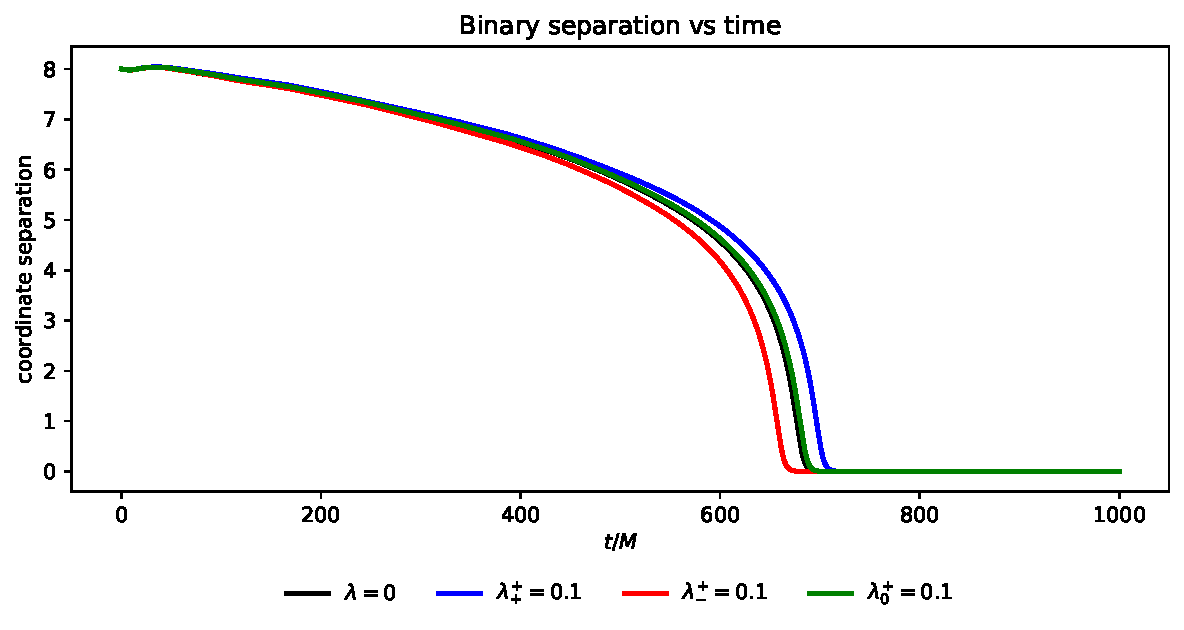
\includegraphics[height=0.22\textheight,keepaspectratio]{Figures/Chapter_2/Q4_spin04_high_charge_separation_comparison.pdf}%
}
\hfill
\subfloat[$q=4$: orbital trajectories.\label{fig:bh_xy_q4}]{%
    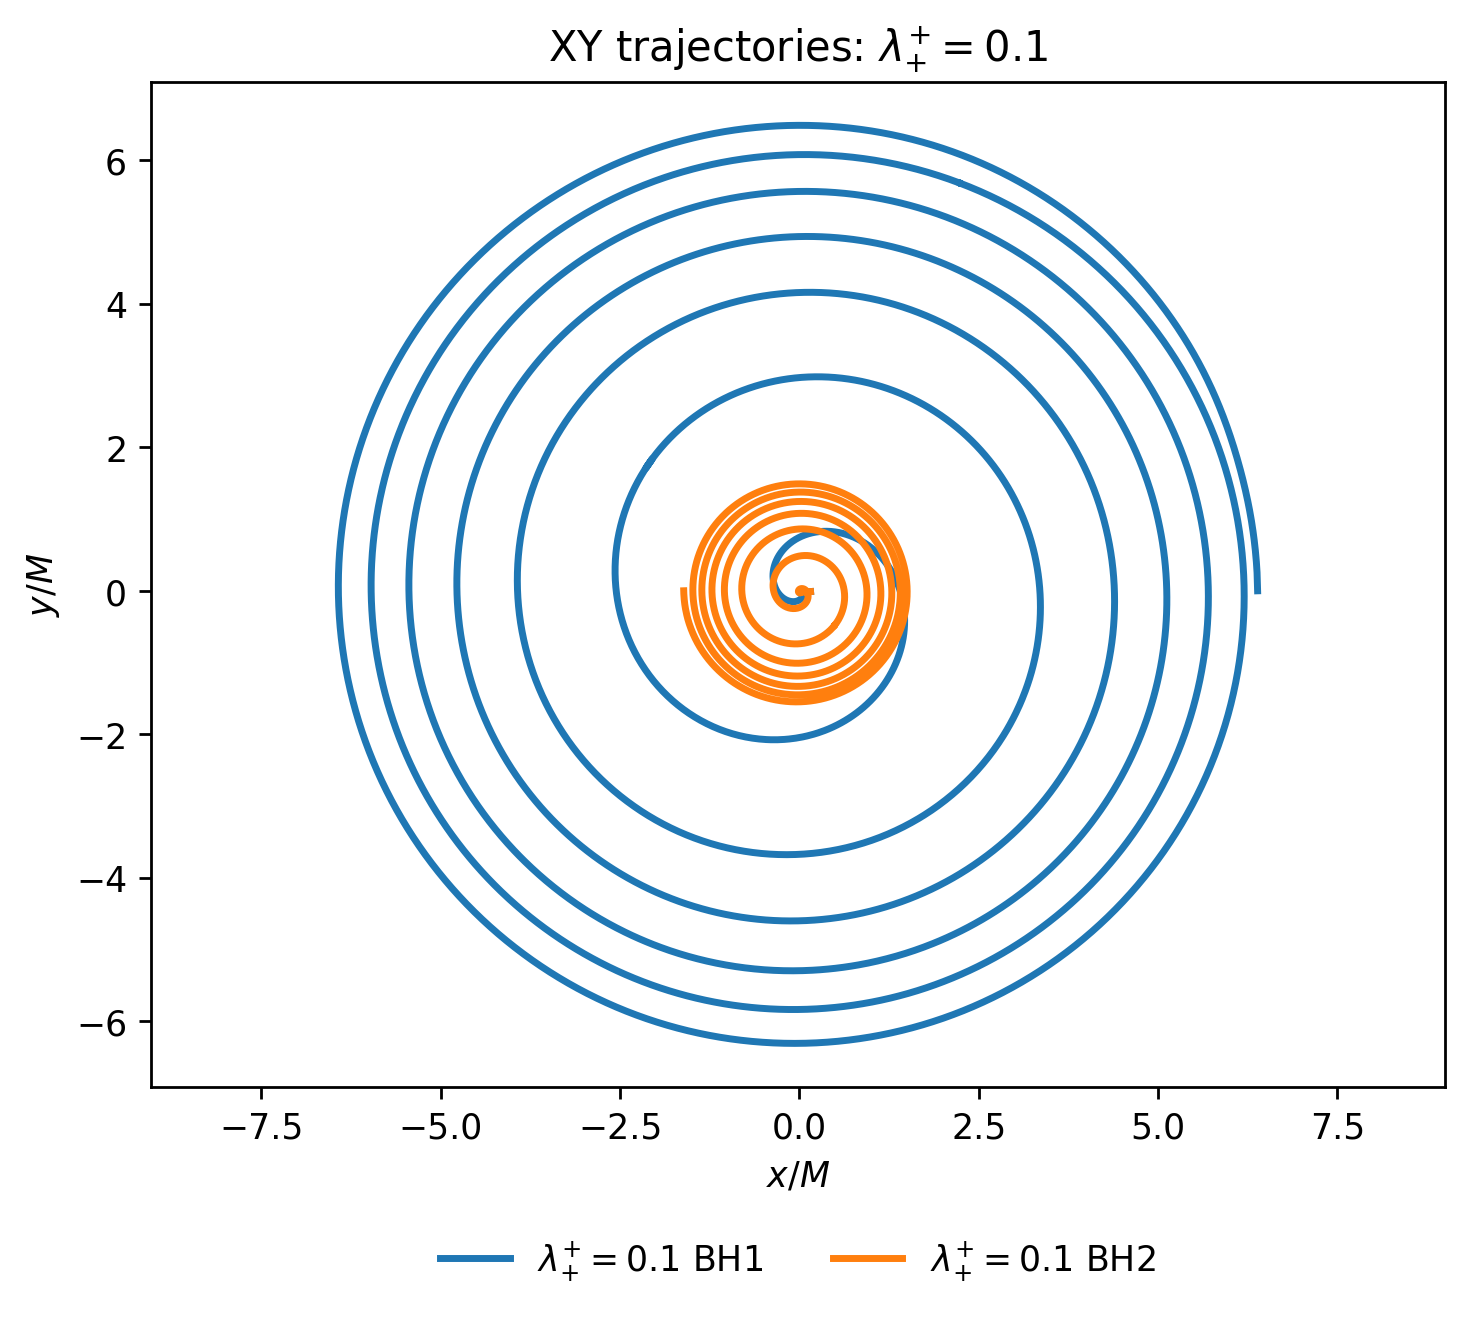
\includegraphics[height=0.22\textheight,keepaspectratio]{Figures/Chapter_2/Q4_spin04_high_charge_Q0p1_pp_xy_trajectory.png}%
}

\vspace{1.0em}

\subfloat[$q=8$: black hole separation.\label{fig:bh_separation_q8}]{%
    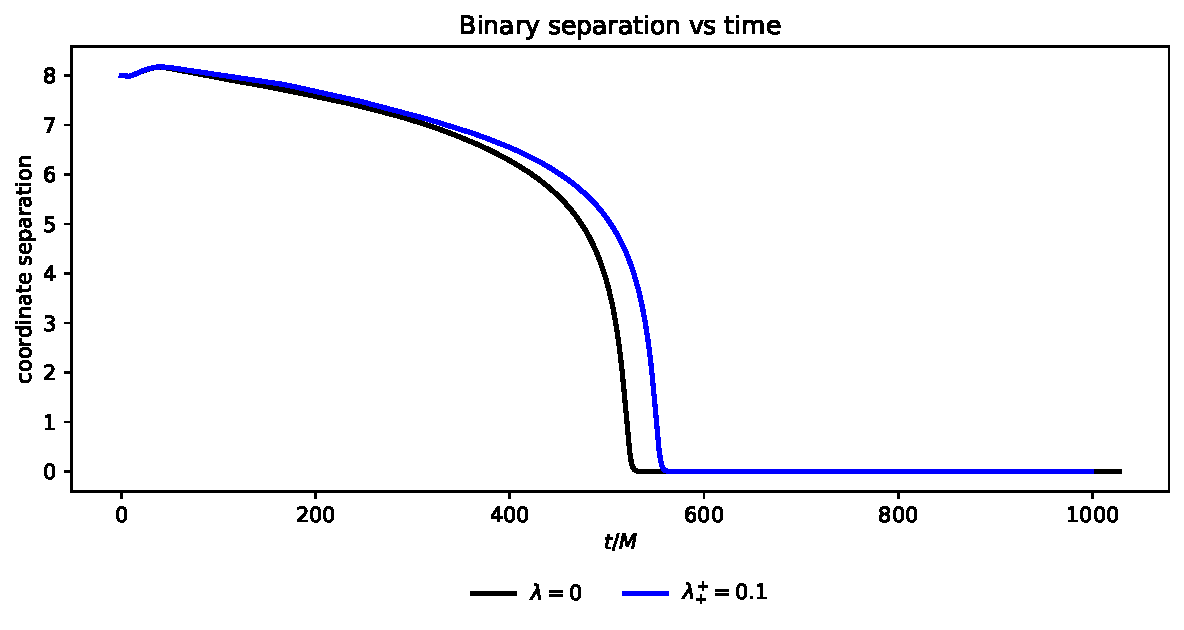
\includegraphics[height=0.22\textheight,keepaspectratio]{Figures/Chapter_2/Q8_SPIN_04_high_charge_separation_comparison.pdf}%
}
\hfill
\subfloat[$q=8$: orbital trajectories.\label{fig:bh_xy_q8}]{%
    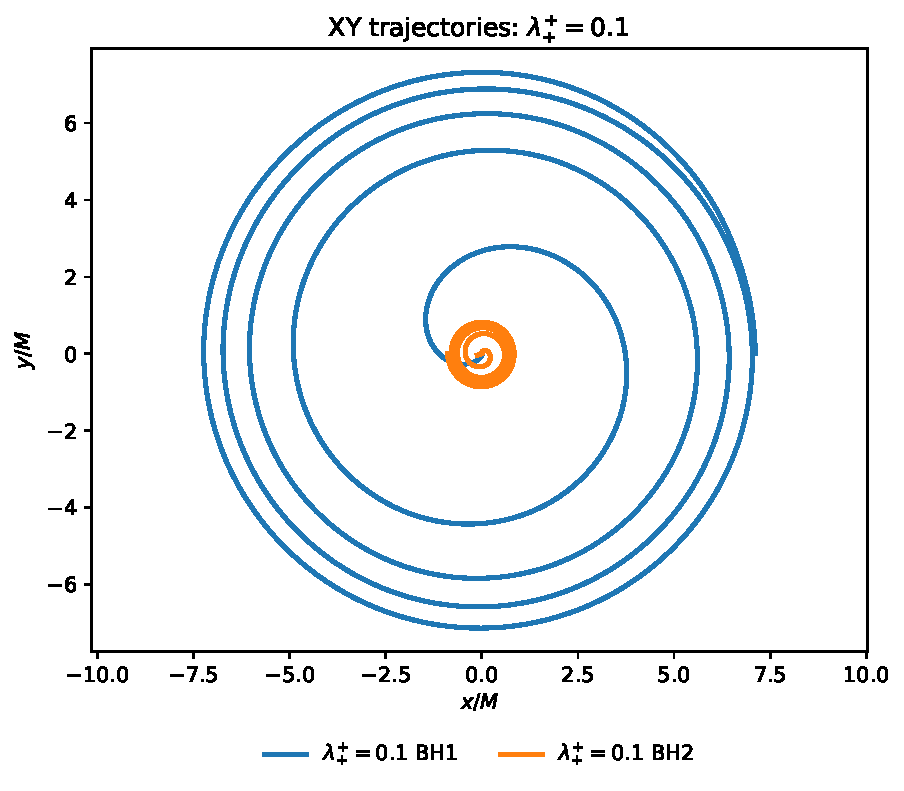
\includegraphics[height=0.22\textheight,keepaspectratio]{Figures/Chapter_2/Q8_SPIN_04_high_charge_Q0p1_pp_xy_trajectory.pdf}%
}

\caption{Orbital dynamics for the $q=4$ and $q=8$ configurations. For each mass ratio, the left panel shows the coordinate separation as a function of time, while the right panel shows representative coordinate trajectories in the orbital plane. The charge configuration affects both the inspiral time and the orbital phasing by modifying the effective interaction between the black holes. The trajectories are approximately quasicircular until the final plunge, which begins once the separation drops below roughly $6M$. Here $\lambda$ denotes the magnitude of the charge-to-mass ratio, $|Q|/M$, assigned to each charged black hole; neutral black holes have $\lambda=0$. The superscript and subscript indicate the charge configuration, with the larger black hole assigned the positive charge. Thus, $\lambda^{+}_{+}$ denotes two positively charged black holes, $\lambda^{+}_{-}$ denotes oppositely charged black holes, and $\lambda^{+}_{0}$ denotes one positively charged and one neutral black hole. The $\lambda=0$ case is the GR reference waveform. In the trajectory plots, orange and blue denote the paths of the heavier and lighter black holes, respectively, with the initial data chosen so that the center of mass is near the origin.}
\label{fig:orbital_dynamics_q4_q8}
\end{figure}
\FloatBarrier
We estimate the orbital eccentricity using an estimator based on the orbital frequency~\cite{RamosBuades2019_EccRed},
\begin{equation}
\varepsilon_{\Omega}(t)
=
\frac{1}{2}
\left[
\frac{\Omega(t)-\Omega_{e=0}(t)}
{\Omega_{e=0}(t)}
\right],
\label{eq:eccentricity_omega_estimator}
\end{equation}
where $\Omega(t)$ is the measured orbital frequency and $\Omega_{e=0}(t)$ denotes the corresponding non-eccentric orbital frequency.

We use an orbital-frequency-based estimator rather than one based directly on the coordinate separation, since separation-based measures can be strongly affected by gauge dynamics, while frequency-based eccentricity estimators are commonly used in eccentricity-reduction procedures \cite{Buonanno2011ReducingEccentricity,Lousto2013OuterLimits}. Although it is still not fully gauge invariant. We track the coordinate positions of each black hole during the inspiral, compute the coordinate separation, and then compute the orbital frequency. The orbital-frequency data are then fit using \verb|NonlinearModelFit| in \verb|Mathematica| with a post-Newtonian-inspired fitting model~\cite{RamosBuades2019_EccRed}.

When fitting the orbital-frequency data, it is useful to include as many orbits as possible in order to reduce the uncertainty in the eccentricity estimate. However, the early part of each simulation contains gauge-settling effects that are not associated with the physical orbital eccentricity, while the late part of the simulation is affected by the onset of plunge. We therefore exclude the first $\sim 200M$ of the simulation and choose the end of the fitting window before the rapid late-inspiral growth of the orbital frequency becomes dominant. In practice, this typically corresponds to ending the fit when the coordinate separation is of order $6M$. The need to have very small eccentricities is balanced by the cost of running runs with higher seperation that need more time to merge.

The measured orbital eccentricities for the catalog runs are shown in Table~\ref{tab:eccentricity_catalog}. The quoted eccentricities are extrapolated from the fit to $t=0M$. The initial coordinate separations are $r=10M$, $r=9M$, and $r=8M$ for the $q=1$, $q=2$, and $q=4$ or $q=8$ configurations, respectively. Most of the lower-spin and lower-charge configurations have eccentricities of order $10^{-3}$, while the largest eccentricities occur in the high-spin and high-charge equal-mass cases.

Figure~\ref{fig:bh_eccentricity} shows an example of the orbital-frequency eccentricity fit for one catalog run. This case has $q=1$, $\chi=0.4$, $\lambda=0.3$, and charge configuration $++$. The fit uses approximately four orbits, with $t_{\mathrm{min}}=200M$ and $t_{\mathrm{max}}=1300M$. The measured eccentricity extrapolated to $t=0M$ is $\varepsilon_\Omega=(14.44\pm0.33)\times10^{-3}$. This comparatively large eccentricity is consistent with the fact that this is a high-charge, like-signed configuration, for which the reduced effective attraction makes the initial momentum prescription less accurate.

In principle, lower eccentricities could be obtained through an iterative eccentricity-reduction procedure, in which the initial momenta are corrected after an initial eccentricity measurement and the simulation is repeated. We do not perform iterative eccentricity reduction for this exploratory catalog. Standard post-Newtonian eccentricity-reduction methods may also need modification in the EMDA case, since the electromagnetic, dilaton, and axion fields can affect the orbital dynamics. Developing eccentricity-reduction procedures that incorporate these effects is left for future work.

\begin{figure}[htbp]
\centering
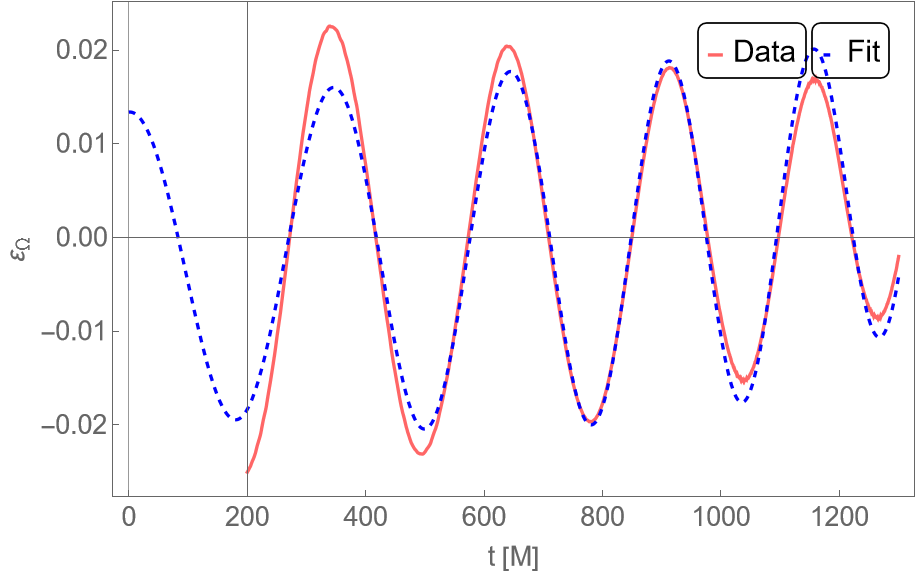
\includegraphics[width=0.48\textwidth]{Figures/Chapter_2/EMDA_eccentricity.png}
\caption{Measured orbital-frequency eccentricity and fitted eccentricity model for a binary black hole inspiral with $q=1$, $\chi=0.4$, $\lambda=0.3$, and charge configuration $++$. The fit is performed from $t_{\mathrm{min}}=200M$ to $t_{\mathrm{max}}=1300M$, excluding early gauge-settling effects and ending before the onset of plunge. The measured eccentricity extrapolated to $t=0M$ is $\varepsilon_\Omega=(14.44\pm0.33)\times10^{-3}$.}
\label{fig:bh_eccentricity}
\end{figure}

% \subsection{Simulation Setup}

\subsection{Waveform mismatch and distinguishability}
\label{sec:waveform_mismatch}

Following Refs.~\cite{Damour1998_ImprovedFilters,Harry2011_TargetedCoherentSearch,Abbott2017_WaveformSystematicsGW150914,Bozzola2021}, we use waveform overlaps and mismatches to quantify differences between the simulated gravitational wave signals.

A direct comparison between charged EMDA and neutral GR waveforms does not, by itself, isolate the contribution of the dilaton and axion fields. Part of the measured difference may arise from the electromagnetic charge and the associated change in the orbital dynamics, rather than from the additional EMDA fields alone. A more complete study would compare EMDA waveforms not only with neutral GR waveforms, but also with charged Einstein--Maxwell evolutions having the same charge configurations. Such a comparison is beyond the scope of the present work. Our goal here is instead to quantify the fixed parameter waveform differences between charged EMDA binaries and their neutral GR counterparts.

To quantify the difference between two gravitational wave signals, we compute the mismatch
\begin{equation}
\mathcal{M}(h_1,h_2)
=
1-\lbrack \max_{\Delta t,\Delta\varphi}\mathcal{O}(h_1,h_2)\rbrack,
\label{eq:mismatch_def}
\end{equation}
where the maximum is taken over relative time shifts $\Delta t$ and polarization-angle shifts $\Delta\varphi$. The overlap $\mathcal{O}$ is defined by
\begin{equation}
\mathcal{O}(h_1,h_2)
=
\frac{(h_1,h_2)}
{\sqrt{(h_1,h_1)(h_2,h_2)}} ,
\label{eq:overlap_def}
\end{equation}
where $(h_1,h_2)$ denotes the detector-noise-weighted inner product between the two waveforms. In practice, this inner product is evaluated over the finite frequency range used in the analysis, with the same preprocessing choices applied to each waveform pair.

The comparison performed here does not maximize over intrinsic binary parameters such as the masses, spins, eccentricity, or charge. These degeneracies could partially obscure the waveform differences found in a fixed parameter comparison and would likely make charge-induced deviations more difficult to identify in a full parameter-estimation study. The mismatch values reported below should therefore be interpreted as a measure of waveform separation at fixed intrinsic parameters, rather than as evidence for a unique observational signature of EMDA theory.

As a rough estimate of distinguishability, we associate a mismatch $\mathcal{M}$ with the critical signal-to-noise ratio
\begin{equation}
\rho_{\rm crit}
\simeq
\frac{1}{\sqrt{2\mathcal{M}}}.
\label{eq:rho_crit}
\end{equation}
This estimate gives the signal-to-noise ratio at which two waveforms with mismatch $\mathcal{M}$ would be expected to become distinguishable in an idealized fixed parameter comparison. 

\section{Results}
\label{sec:results}

We compare charged EMDA waveforms with neutral GR reference waveforms for a representative set of binary black hole configurations. The purpose of this comparison is to determine how the waveform differences depend on charge magnitude, charge configuration, mass ratio, and spin. In each case, the charged EMDA waveform is compared against a neutral reference waveform with the same mass ratio and spin.

The simulation catalog considered in this chapter is summarized in Table~\ref{tab:simulation_catalog}. For each choice of mass ratio $q=m_1/m_2$, spin $\chi$, and charge magnitude $\lambda=|Q|/M$, we consider one neutral configuration, $Q_1=Q_2=0$, and several charged configurations. We label the charged cases by the signs of the two black hole charges. The cases $++$, $+-$, and $+0$ denote similar charges, oppositely signed charges, and a configuration with one charged and one neutral black hole, respectively. For unequal-mass binaries, the larger black hole is assigned the positive charge in the $+-$ and $+0$ cases.

Representative peak-aligned waveforms are shown in Fig.~\ref{fig:peak_aligned_hplus_all_mass_ratios}. The figure compares the strain component $r h_+$ for selected charged EMDA configurations against the corresponding neutral GR reference waveform. The waveforms are aligned at the peak amplitude in order to emphasize differences in the late inspiral, merger, and ringdown. Even after this alignment, the charged and neutral waveforms show visible phase and amplitude differences, indicating that charge and the additional EMDA fields can modify the binary dynamics prior to merger as well as the waveform near peak emission.

\begin{figure*}[t]
\centering

\subfloat[$q=1$.\label{fig:q1_peak_aligned_hplus}]{%
    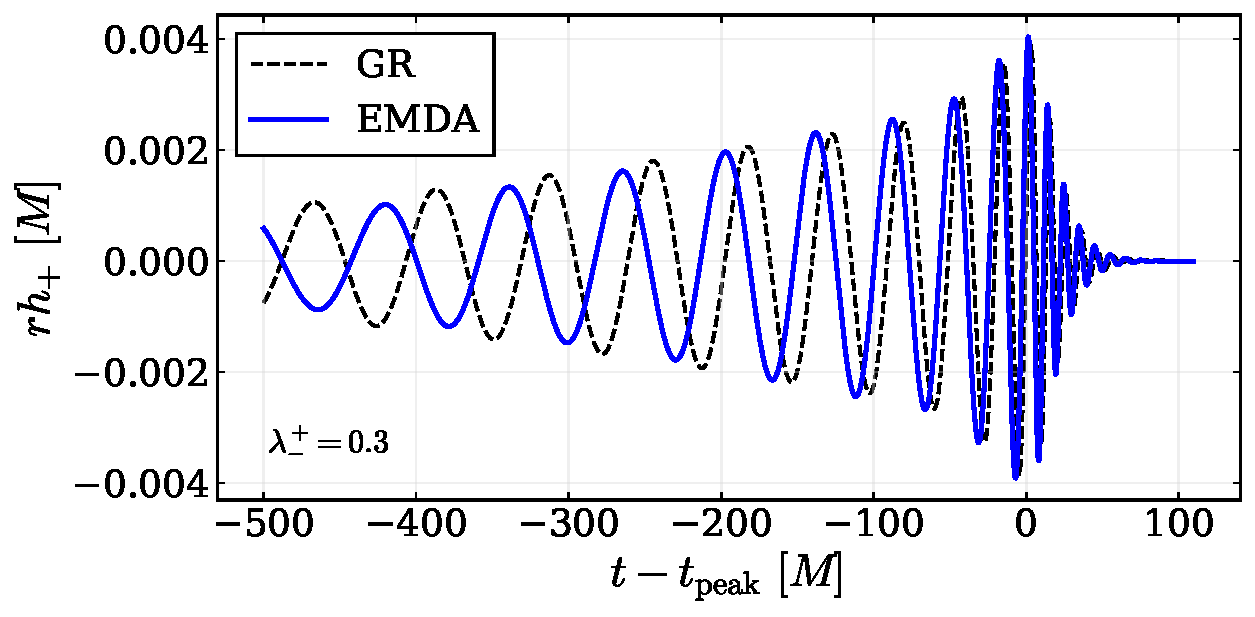
\includegraphics[width=0.48\textwidth]{Figures/Chapter_2/q1_Q0_vs_Q0p15_pn_peak_aligned_hplus_notitle.pdf}%
}
\hfill
\subfloat[$q=2$.\label{fig:q2_peak_aligned_hplus}]{%
    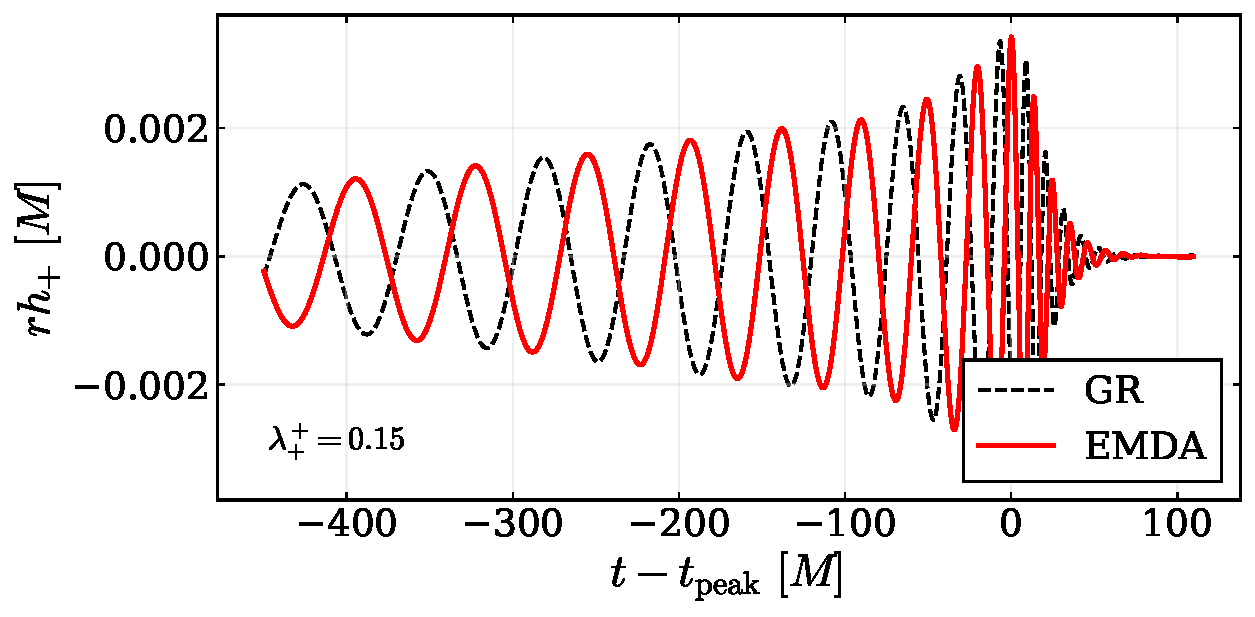
\includegraphics[width=0.48\textwidth]{Figures/Chapter_2/q2_Q0_vs_Q0p15_pp_peak_aligned_hplus_notitle.pdf}%
}

\vspace{0.5em}

\subfloat[$q=4$.\label{fig:q4_peak_aligned_hplus}]{%
    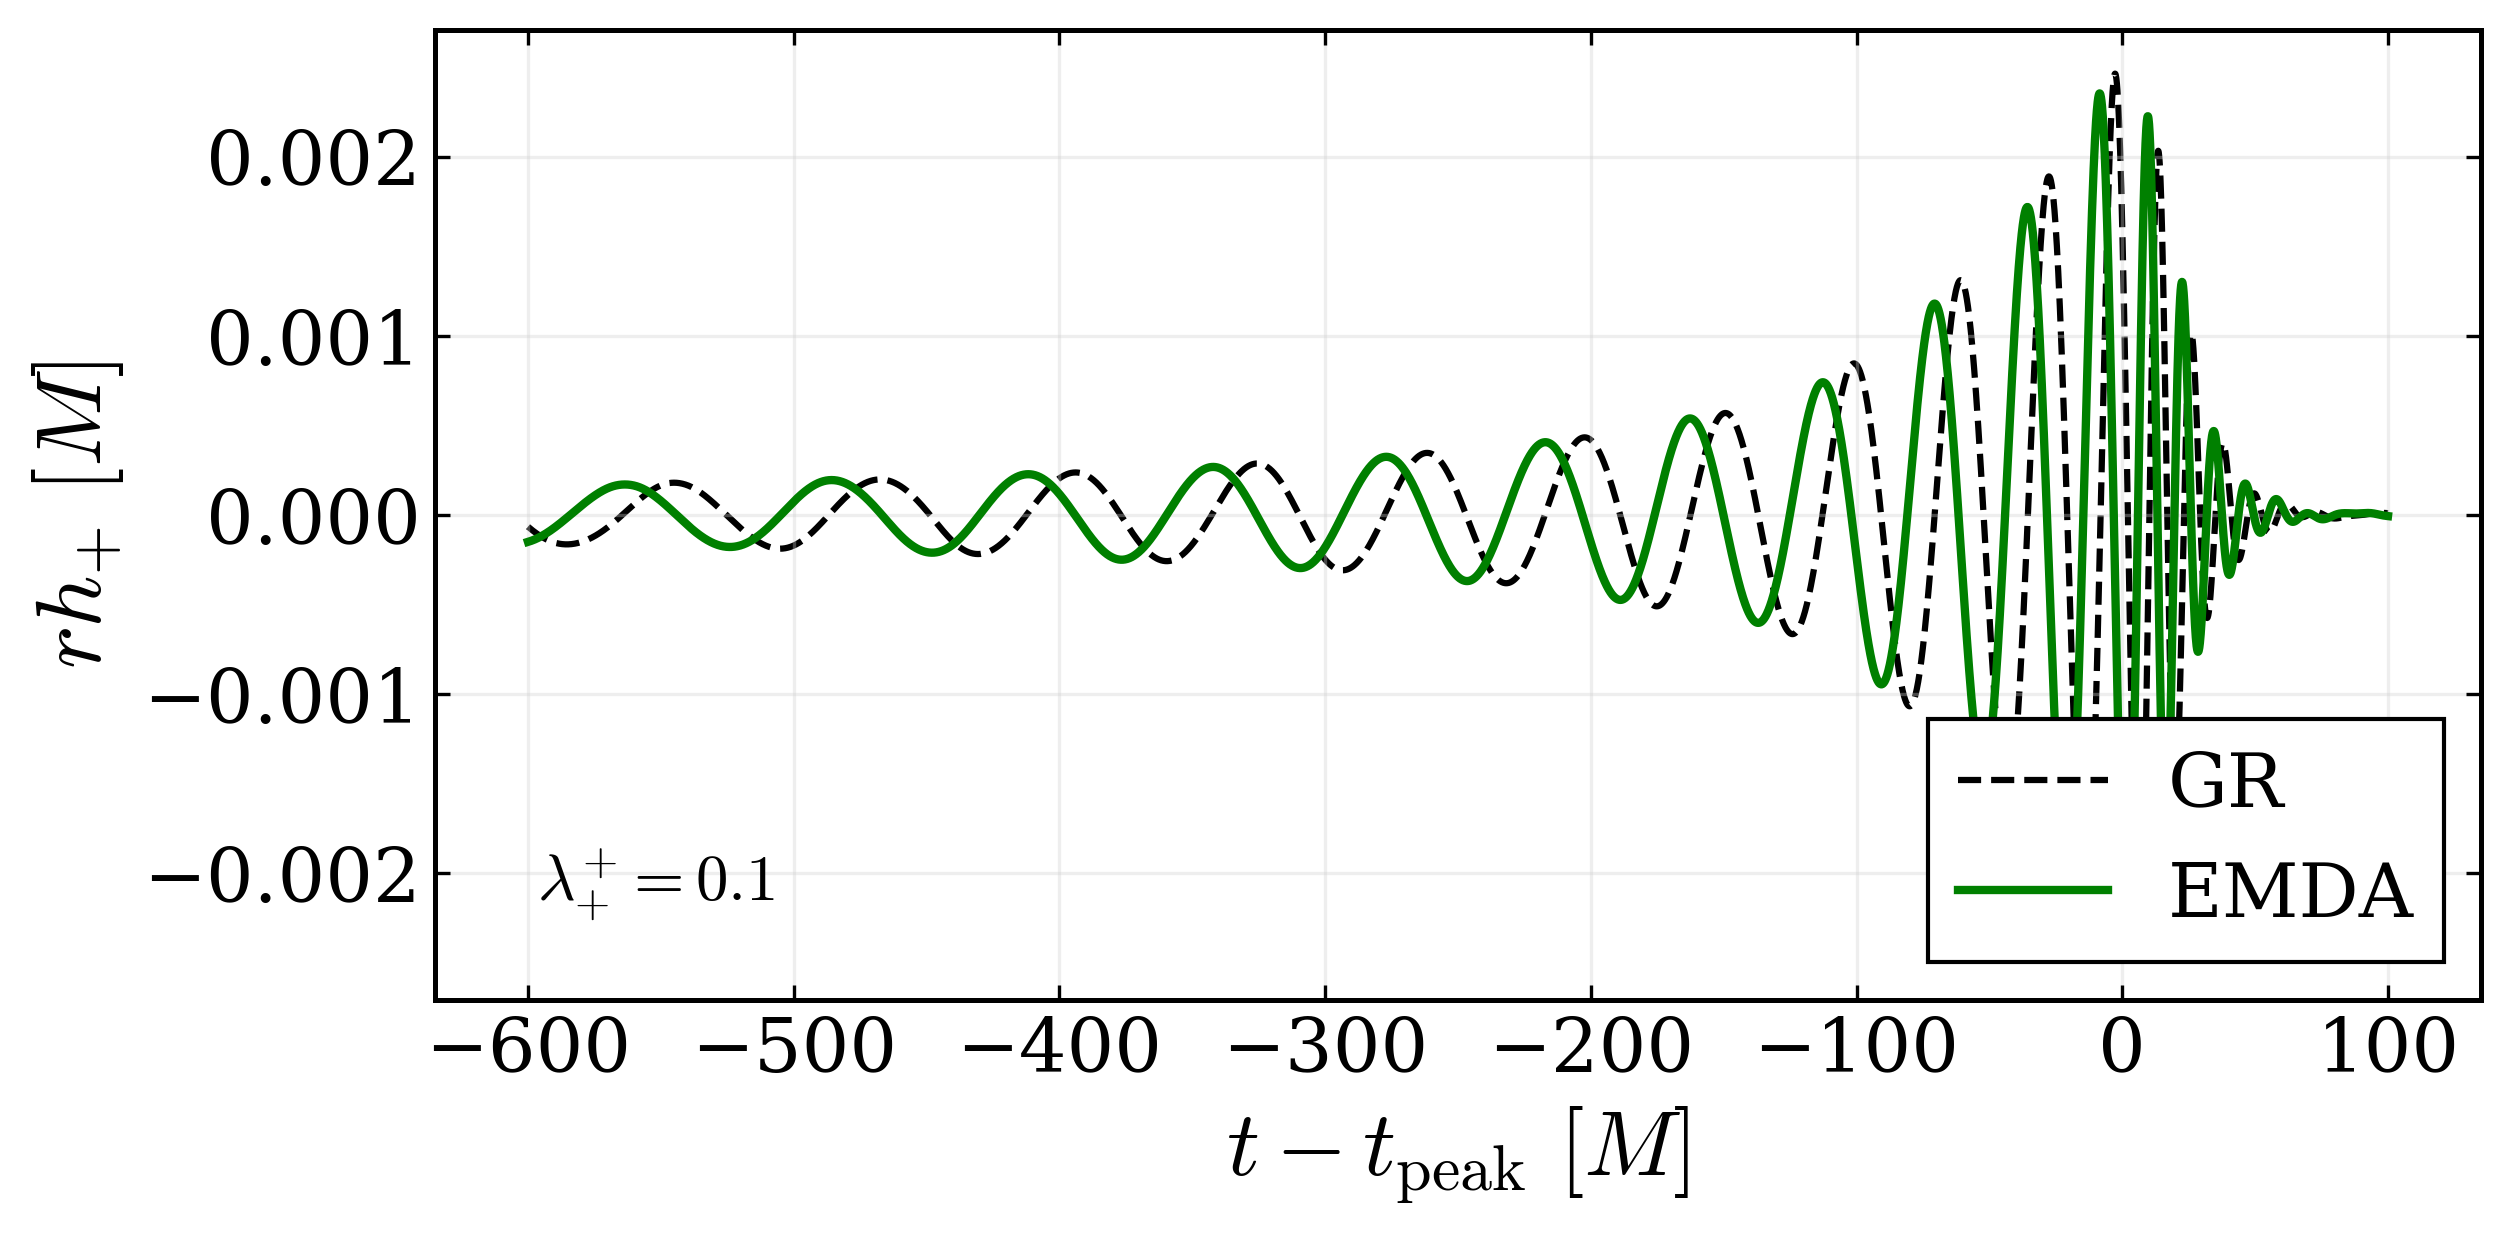
\includegraphics[width=0.48\textwidth]{Figures/Chapter_2/Q0_vs_Q0p1_pp_peak_aligned_hplus_notitle.png}%
}
\hfill
\subfloat[$q=8$.\label{fig:q8_peak_aligned_hplus}]{%
    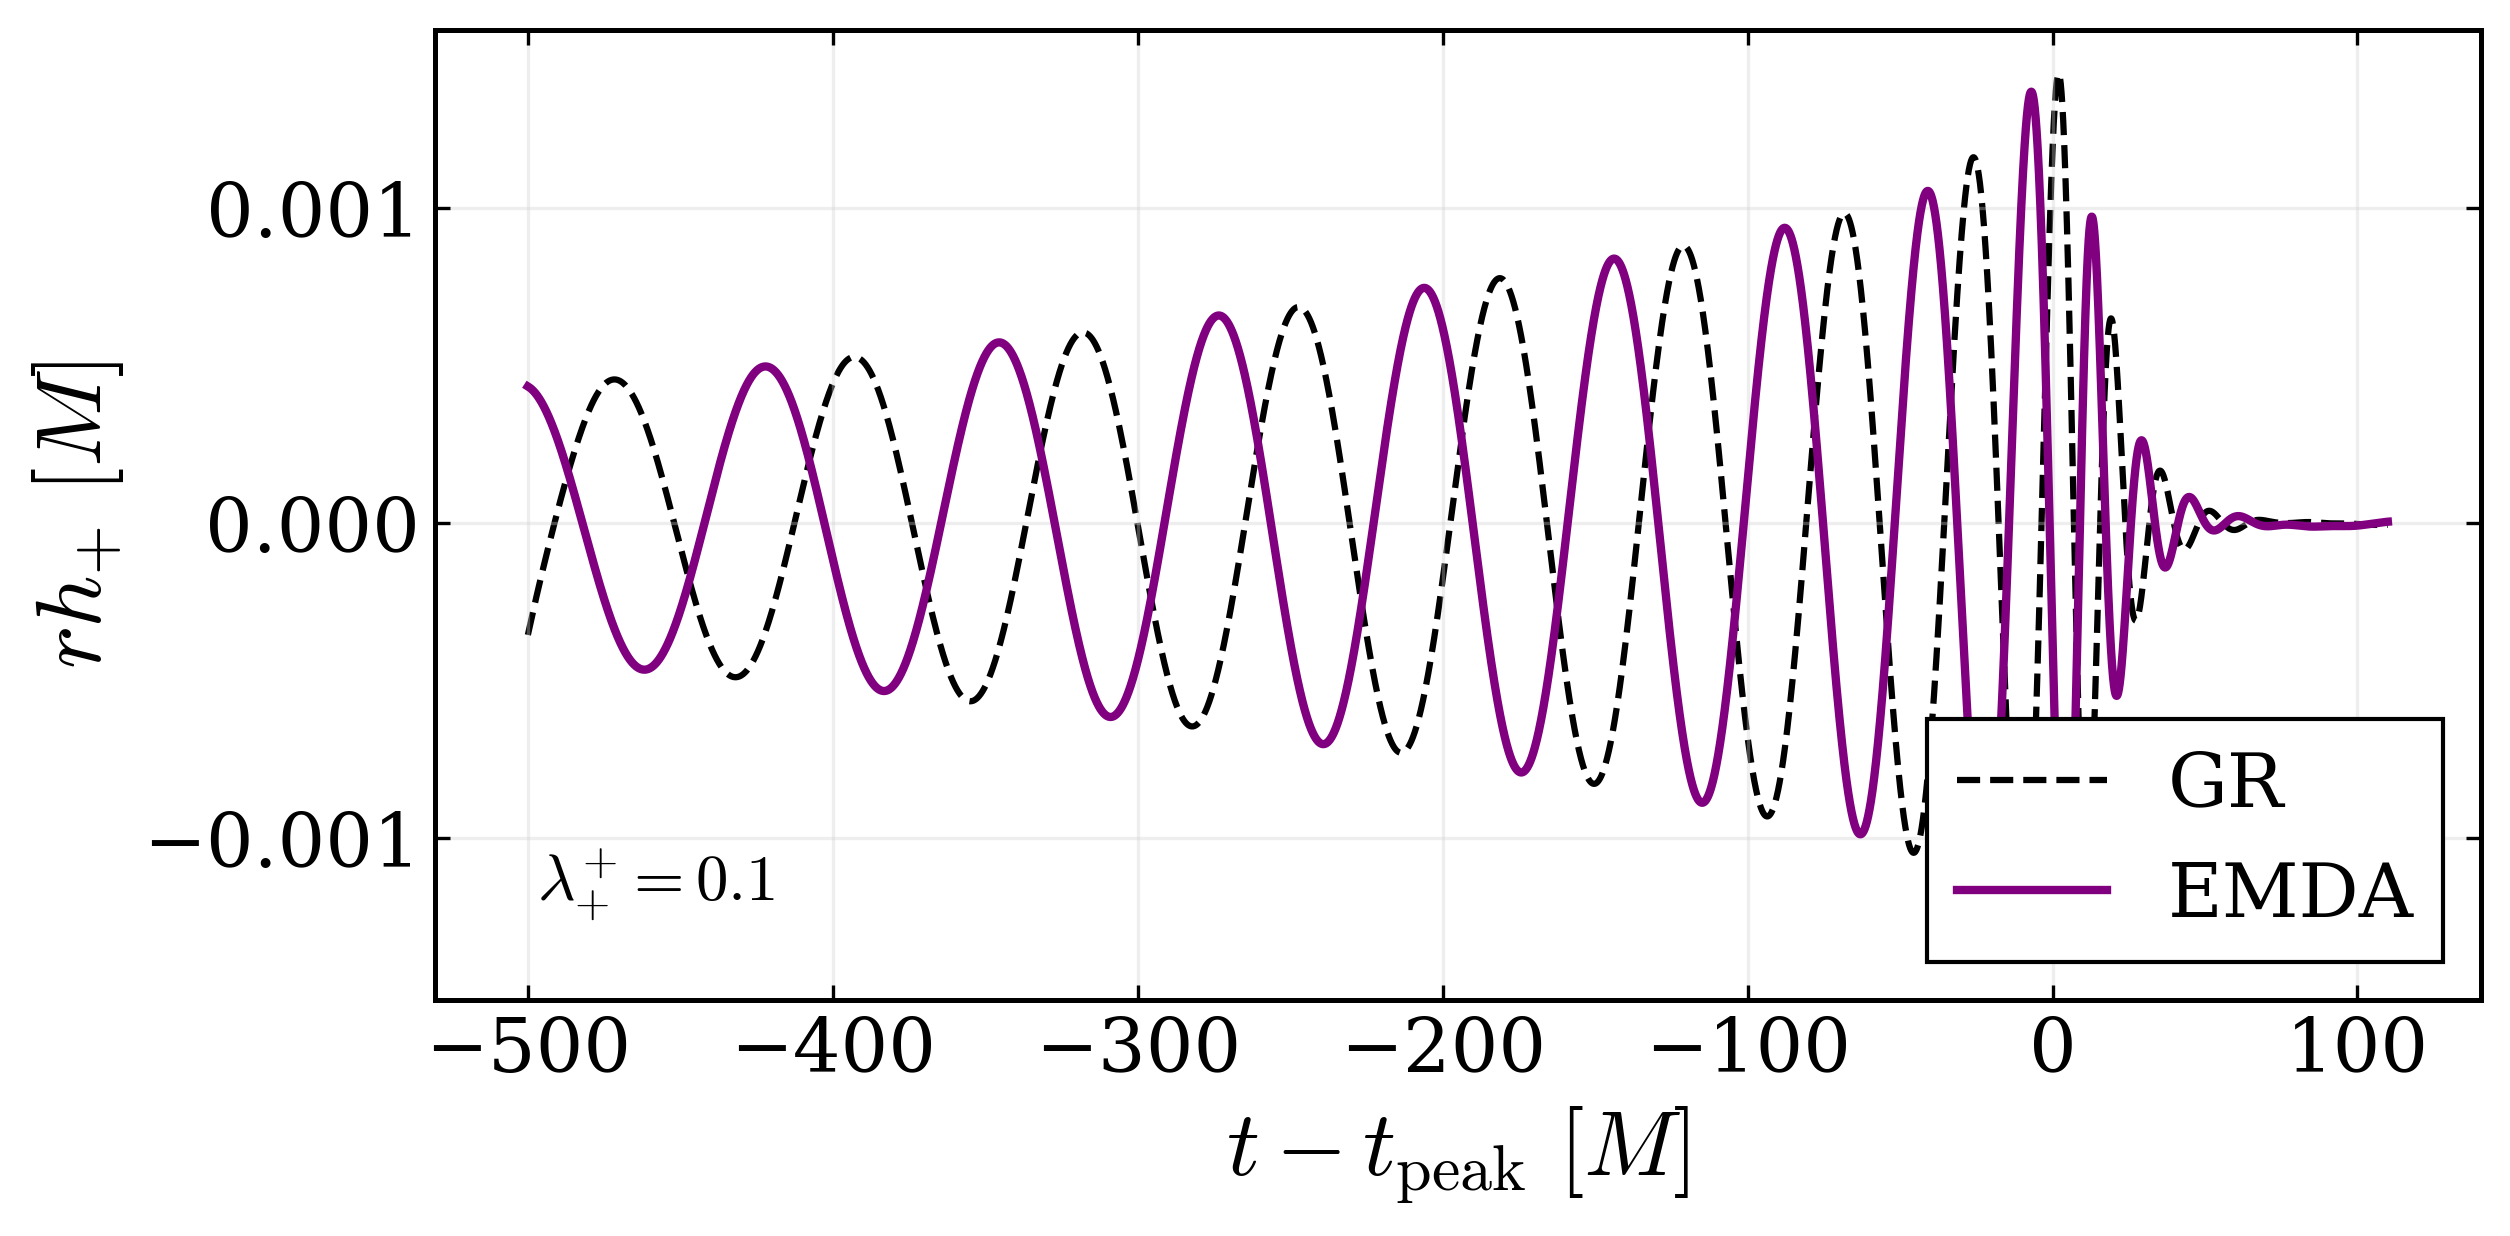
\includegraphics[width=0.48\textwidth]{Figures/Chapter_2/q8_Q0_vs_Q0p1_pp_peak_aligned_hplus_notitle.png}%
}

\caption{Peak-aligned comparisons of the gravitational wave strain component $r h_{+}$ for representative charged EMDA configurations against the corresponding neutral GR reference waveforms. In each panel, the time coordinate is shifted so that the waveform peak occurs at $t-t_{\mathrm{peak}}=0$. The remaining differences after peak alignment reflect changes in the accumulated phase, merger time, and waveform morphology.}
\label{fig:peak_aligned_hplus_all_mass_ratios}

\end{figure*}

The full set of waveform mismatches is computed using the numerical-relativity analysis toolkit \texttt{kuibit}~\cite{kuibit}. kuibit is a numerical relativity library with functions to process gravitational waves.  The results are given in Table~\ref{tab:waveform_mismatches_combined}. The mismatch values generally increase with charge magnitude, although the trend is not monotonic across all spin and charge configurations. For example, in the $q=1$, $\chi=0.4$, $++$ sequence, the mismatch increases from $2.60\times10^{-4}$ for $\lambda=0.1$ to $5.28\times10^{-3}$ for $\lambda=0.3$. Similar growth with charge is seen in several other equal-mass configurations.

The charge configuration also plays an important role. The $++$, $+-$, and $+0$ cases do not produce equivalent waveform differences, even at the same charge magnitude. In many cases, the singly charged $+0$ configurations remain closer to the neutral reference waveform than the corresponding two-charged configurations. This is consistent with the expectation that the strength and symmetry of the charge distribution influence both the orbital dynamics and the matter-field content of the spacetime. Oppositely signed charges can also produce comparatively large mismatches, since the electromagnetic interaction increases the effective attraction and changes the inspiral rate.

The $\chi=0.8$ equal-mass configurations are somewhat anomalous compared with the lower-spin cases. While the mismatch generally grows with charge for the lower-spin sequences, the $\chi=0.8$ cases show larger and less monotonic variations across the different charge configurations. These runs also have noticeably larger eccentricities, especially at the highest charge magnitudes, suggesting that the approximate charged initial-data prescription is being pushed beyond the regime where it gives uniformly low-eccentricity inspirals. We therefore include these cases as useful indicators of where large waveform differences can occur, but we do not interpret their detailed mismatch hierarchy as a clean physical trend.

The high-spin configurations nevertheless show the largest waveform separations in the catalog. For the $q=1$, $\chi=0.8$ cases, some mismatches reach the $10^{-2}$--$10^{-1}$ level. These large values indicate that the charged and neutral waveforms are substantially separated at fixed intrinsic parameters. However, because these cases are also more sensitive to eccentricity and initial-data systematics, they should not be interpreted as isolated signatures of the dilaton or axion fields.

The critical signal-to-noise ratio estimate associated with the mismatch values spans approximately $\rho_{\rm crit}\sim2.3$ to over 500 across the catalog. These values should be understood as fixed parameter distinguishability estimates: they indicate the signal-to-noise ratio at which the charged EMDA waveform and the corresponding neutral GR waveform would become distinguishable if the intrinsic binary parameters were held fixed. In a full parameter-estimation study, changes in the masses, spins, eccentricity, or other parameters could partially obscure these differences. The mismatch values therefore quantify waveform separation within this catalog, rather than providing direct observational bounds on EMDA theory.

These results demonstrate that our EMDA evolution framework can produce a range of charged binary black hole simulations with relatively low eccentricity. For most of the catalog, the observed waveform trends are consistent with physical expectations: increasing the charge magnitude tends to increase the waveform mismatch, and different charge configurations produce distinct inspiral and merger behavior. Nevertheless, the highest-spin configurations require additional caution. These cases show larger residual eccentricities and noisier waveforms than the lower-spin runs, suggesting that the approximate charged initial-data prescription and the chosen grid resolution may be less reliable in this region of parameter space. Future work should revisit these cases with improved eccentricity reduction and higher-resolution simulations to determine whether the large waveform differences remain after these numerical effects are better controlled.
\section{Conclusion}
\label{sec:conclusion}

In this chapter, we presented an exploratory waveform catalog for charged binary black hole simulations in Einstein--Maxwell--dilaton--axion (EMDA) theory. We compared the resulting charged EMDA waveforms with neutral general-relativistic reference waveforms having the same mass ratio and spin. Across much of the catalog, the waveform differences increase with the charge magnitude, indicating that charge and the additional EMDA fields can produce appreciable changes in the gravitational wave signal. The trend is clearest in the lower-spin configurations, while the highest-spin cases show larger and less monotonic differences that are likely more sensitive to eccentricity and the approximate charged initial-data prescription.

Using the mismatch as a rough fixed parameter distinguishability estimate, the largest waveform separations in the catalog correspond to critical signal-to-noise ratios, with the smallest values approximately $\rho_{\rm crit}\sim2.3$. These values indicate that the largest charged EMDA deviations from the corresponding neutral GR waveforms are substantial at fixed intrinsic parameters. However, they should not be interpreted as direct observational thresholds or constraints on EMDA theory. A full parameter-estimation study would be required to determine whether these differences could be mimicked by changes in the masses, spins, eccentricity, total mass scale, or other binary parameters.

The waveform differences found here should also be interpreted with care because the comparison is made against neutral GR rather than against charged Einstein--Maxwell binaries. As a result, the reported mismatches include the combined effect of electric charge, modified orbital dynamics, and the additional dilaton and axion fields. They cannot be attributed uniquely to the dilaton or axion fields alone. A more complete comparison would include corresponding Einstein--Maxwell simulations with the same charge configurations, allowing the purely electromagnetic contribution to be separated from the additional EMDA-field effects.

These results demonstrate that EMDA theory provides a useful numerical-relativity testbed for studying charged beyond-GR effects in binary black hole mergers. Even within this exploratory catalog, charged EMDA binaries can produce waveform differences that are large enough to motivate further study. Natural next steps include larger parameter surveys, improved charged initial data, iterative eccentricity reduction, longer inspirals, and convergence studies of the waveform mismatches. It would be especially useful to extend the high-mass-ratio portion of the catalog by performing additional $q=8$ simulations with the full set of charge configurations, higher spins, and larger charge magnitudes. Direct comparisons among neutral GR, charged Einstein--Maxwell, and charged EMDA binaries would also help separate ordinary electromagnetic effects from waveform changes associated specifically with the dilaton and axion fields.
\section{Simulation Catalog}
\label{sec:simulation_catalog}

The simulations used in this chapter are summarized in Table~\ref{tab:simulation_catalog}. The catalog samples several mass ratios, spin values, charge magnitudes, and charge configurations. For each mass ratio and spin, we include a neutral reference simulation and compare the charged EMDA evolutions against that corresponding neutral case.
\FloatBarrier
\begin{table*}[htbp]
\centering
\caption{EMDA binary black hole simulation catalog. Here $q=m_1/m_2$ denotes the mass ratio, $\chi$ denotes the dimensionless spin parameter, and $\lambda_i=Q_i/M_i$ denotes the charge-to-mass ratio of black hole $i$. The neutral case corresponds to $Q_1=Q_2=0$. For charged configurations, the magnitude of the nonzero charge-to-mass ratios is denoted by $\lambda$, with the sign structure indicated by the charge configuration. The configurations $++$, $+-$, and $+0$ denote like-signed charges, oppositely signed charges, and cases in which only one black hole is charged, respectively. Because the neutral configuration is independent of $\lambda$, it is listed only once for each mass ratio and spin.}
\label{tab:simulation_catalog}
\begin{tabular}{ccccccc}
\toprule
Mass Ratio $q$ & Spin $\chi$ & Charge Magnitude $\lambda$ & Neutral & $++$ & $+-$ & $+0$ \\
\midrule
1 & 0.0 & 0.1 & $\checkmark$ & $\checkmark$ & $\checkmark$ & $\checkmark$ \\
1 & 0.0 & 0.2 & -- & $\checkmark$ & $\checkmark$ & $\checkmark$ \\
1 & 0.0 & 0.3 & -- & $\checkmark$ & $\checkmark$ & $\checkmark$ \\
\midrule
1 & 0.4 & 0.1 & $\checkmark$ & $\checkmark$ & $\checkmark$ & $\checkmark$ \\
1 & 0.4 & 0.2 & -- & $\checkmark$ & $\checkmark$ & $\checkmark$ \\
1 & 0.4 & 0.3 & -- & $\checkmark$ & $\checkmark$ & $\checkmark$ \\
\midrule
1 & 0.8 & 0.1 & $\checkmark$ & $\checkmark$ & $\checkmark$ & $\checkmark$ \\
1 & 0.8 & 0.2 & -- & $\checkmark$ & $\checkmark$ & $\checkmark$ \\
1 & 0.8 & 0.3 & -- & $\checkmark$ & $\checkmark$ & $\checkmark$ \\
\midrule
2 & 0.0 & 0.05 & $\checkmark$ & $\checkmark$ & $\checkmark$ & $\checkmark$ \\
2 & 0.0 & 0.15 & -- & $\checkmark$ & $\checkmark$ & $\checkmark$ \\
\midrule
2 & 0.4 & 0.05 & $\checkmark$ & $\checkmark$ & $\checkmark$ & $\checkmark$ \\
2 & 0.4 & 0.15 & -- & $\checkmark$ & $\checkmark$ & $\checkmark$ \\
\midrule
4 & 0.4 & 0.05 & $\checkmark$ & $\checkmark$ & $\checkmark$ & $\checkmark$ \\
4 & 0.4 & 0.10 & -- & $\checkmark$ & $\checkmark$ & $\checkmark$ \\
\midrule
8 & -0.2 & 0.10 & $\checkmark$ & $\checkmark$ & -- & -- \\
\bottomrule
\end{tabular}
\end{table*}
The simulations used in this chapter are summarized in Table~\ref{tab:simulation_catalog}. The catalog samples several mass ratios, spin values, charge magnitudes, and charge configurations. For each mass ratio and spin, we include a neutral reference simulation and compare the charged EMDA evolutions against that corresponding neutral case. For the $q=8$ simulations, we choose a negative spin value, $\chi=-0.2$, corresponding to spin anti-aligned with the orbital angular momentum. This choice reduces the inspiral time relative to an aligned-spin configuration, making the high-mass-ratio simulations less computationally expensive.
\FloatBarrier
\begin{table*}[t]
\centering
\caption{Mismatch of charged EMDA binary black hole waveforms relative to the corresponding neutral reference waveform \texttt{Q0}. Here $q=m_1/m_2$, $\chi$ is the dimensionless spin parameter, and $\lambda_i=Q_i/M_i$. The column $|\lambda_i|$ gives the magnitude of the nonzero charge-to-mass ratio used in each charged configuration. The columns $++$, $+-$, and $+0$ denote like-signed charges, oppositely signed charges, and configurations in which only one black hole is charged, respectively. The mismatch is computed from the $(\ell,m)=(2,2)$ gravitational waveform using the numerical-relativity analysis package \texttt{kuibit}, after optimizing over relative time and polarization shifts. The values in parentheses give the approximate fixed parameter critical signal-to-noise ratio, $\rho_{\rm crit}\simeq 1/\sqrt{2\mathcal{M}}$. These values should be interpreted as rough waveform-separation estimates rather than full observational detection thresholds.}
\label{tab:waveform_mismatches_combined}
\scriptsize
\setlength{\tabcolsep}{4pt}
\renewcommand{\arraystretch}{1.08}
\resizebox{\textwidth}{!}{%
\begin{tabular}{cccccc}
\toprule
Mass Ratio $q$ & Spin $\chi$ & Charge Magnitude $|\lambda_i|$
& $++$ & $+-$ & $+0$ \\
\midrule
1 & 0.0 & 0.10 & $3.53\times 10^{-4};(37.6)$ & $2.74\times 10^{-4};(42.8)$ & $1.55\times 10^{-4};(56.8)$ \\
1 & 0.0 & 0.20 & $6.71\times 10^{-4};(27.3)$ & $1.45\times 10^{-3};(18.5)$ & $6.91\times 10^{-4};(26.9)$ \\
1 & 0.0 & 0.30 & $1.94\times 10^{-3};(16.0)$ & $5.32\times 10^{-3};(9.7)$ & $7.54\times 10^{-4};(25.8)$ \\
\midrule
1 & 0.4 & 0.10 & $2.60\times 10^{-4};(43.9)$ & $2.87\times 10^{-4};(41.8)$ & $4.08\times 10^{-4};(35.0)$ \\
1 & 0.4 & 0.20 & $7.10\times 10^{-4};(26.5)$ & $7.40\times 10^{-3};(8.2)$ & $7.42\times 10^{-4};(26.0)$ \\
1 & 0.4 & 0.30 & $5.28\times 10^{-3};(9.7)$ & $2.90\times 10^{-2};(4.1)$ & $1.04\times 10^{-3};(21.9)$ \\
\midrule
1 & 0.8 & 0.10 & $2.77\times 10^{-4};(42.5)$ & $9.44\times 10^{-4};(23.0)$ & $1.03\times 10^{-3};(22.0)$ \\
1 & 0.8 & 0.20 & $4.66\times 10^{-2};(3.3)$ & $9.30\times 10^{-2};(2.3)$ & $1.67\times 10^{-2};(5.5)$ \\
1 & 0.8 & 0.30 & $6.19\times 10^{-2};(2.8)$ & $2.53\times 10^{-2};(4.4)$ & $7.99\times 10^{-3};(7.9)$ \\
\midrule
2 & 0.0 & 0.05 & $1.58\times 10^{-3};(17.8)$ & $1.34\times 10^{-3};(19.3)$ & $2.56\times 10^{-5};(139.7)$ \\
2 & 0.0 & 0.15 & $1.83\times 10^{-3};(16.5)$ & $3.21\times 10^{-3};(12.5)$ & $7.47\times 10^{-4};(25.9)$ \\
\midrule
2 & 0.4 & 0.05 & $7.27\times 10^{-5};(82.9)$ & $1.33\times 10^{-4};(61.3)$ & $1.73\times 10^{-6};(537.4)$ \\
2 & 0.4 & 0.15 & $6.17\times 10^{-4};(28.5)$ & $2.34\times 10^{-4};(46.2)$ & $7.58\times 10^{-5};(81.2)$ \\
\midrule
4 & 0.4 & 0.05 & $5.10\times 10^{-5};(99.0)$ & $7.34\times 10^{-5};(82.5)$ & $7.17\times 10^{-5};(83.5)$ \\
4 & 0.4 & 0.10 & $3.17\times 10^{-4};(39.7)$ & $1.82\times 10^{-4};(52.5)$ & $8.80\times 10^{-5};(75.4)$ \\
\midrule
8 & -0.2 & 0.10 & $1.14\times 10^{-3};(21.0)$ & \text{--} & \text{--} \\
\bottomrule
\end{tabular}%
}
\end{table*}
Table~\ref{tab:waveform_mismatches_combined} summarizes the fixed parameter waveform mismatches between the charged EMDA simulations and the corresponding neutral reference waveforms. Across much of the catalog, the mismatch increases with charge magnitude, although the trend is not strictly monotonic for every spin and charge configuration. The clearest growth occurs in the equal-mass lower-spin cases. For example, for $q=1$ and $\chi=0.4$, the $++$ mismatch grows from $2.60\times10^{-4}$ at $\lambda=0.1$ to $5.28\times10^{-3}$ at $\lambda=0.3$, while the $+-$ mismatch grows even more strongly, reaching $2.90\times10^{-2}$. The charge configuration also has a significant effect: the $+0$ cases are often closer to the neutral reference waveform than the two-charged configurations, while the $+-$ cases can produce relatively large mismatches because the opposite charges increase the effective attraction and accelerate the inspiral. The largest mismatches occur in the high-spin $q=1$, $\chi=0.8$ cases, where some values reach the $10^{-2}$--$10^{-1}$ level; however, these cases should be interpreted with caution because they also have larger residual eccentricities and noisier waveforms. For the unequal-mass cases, especially $q=2$ and $q=4$, the mismatches are generally smaller, with many values below $10^{-3}$. Overall, the table shows that charge can produce measurable waveform differences at fixed mass ratio and spin, but that the size of the effect depends strongly on charge magnitude, charge configuration, and spin.
\section{Measured Eccentricities}
\label{sec:measured_eccentricities}

Table~\ref{tab:eccentricity_catalog} summarizes the measured orbital eccentricities for the EMDA waveform catalog. The values are obtained from the orbital-frequency eccentricity estimator described in Sec.~\ref{sec:eccentricity_control} and are reported as $(\varepsilon_\Omega \pm \delta\varepsilon_\Omega)\times10^3$.

\begin{table*}[htbp]
\centering
\caption{Measured orbital eccentricities for the EMDA waveform catalog. The entries are reported as $(\varepsilon_\Omega \pm \delta\varepsilon_\Omega)\times10^3$. Here $q=m_1/m_2$ denotes the mass ratio, $\chi$ denotes the dimensionless spin parameter, and $\lambda_i=Q_i/M_i$ denotes the charge-to-mass ratio of black hole $i$. The neutral case corresponds to $Q_1=Q_2=0$. For charged configurations, the magnitude of the nonzero charge-to-mass ratios is denoted by $\lambda$, with the sign structure indicated by the charge configuration. The configurations $++$, $+-$, and $+0$ denote like-signed charges, oppositely signed charges, and cases in which only one black hole is charged, respectively.}
\label{tab:eccentricity_catalog}
\begin{tabular}{ccccccc}
\toprule
Mass Ratio $q$ & Spin $\chi$ & Charge Magnitude $\lambda$ & Neutral & $++$ & $+-$ & $+0$ \\
\midrule
1 & 0.0 & 0.10 & $1.59 \pm 0.21$ & $2.57 \pm 0.17$ & $1.97 \pm 0.27$ & $2.54 \pm 0.23$ \\
1 & 0.0 & 0.20 & -- & $6.26 \pm 0.26$ & $3.52 \pm 0.35$ & $4.41 \pm 0.24$ \\
1 & 0.0 & 0.30 & -- & $14.99 \pm 0.40$ & $2.08 \pm 0.36$ & $5.28 \pm 0.45$ \\
\midrule
1 & 0.4 & 0.10 & $1.39 \pm 0.10$ & $1.80 \pm 0.11$ & $1.30 \pm 0.13$ & $1.26 \pm 0.11$ \\
1 & 0.4 & 0.20 & -- & $5.17 \pm 0.18$ & $1.04 \pm 0.22$ & $2.68 \pm 0.18$ \\
1 & 0.4 & 0.30 & -- & $14.44 \pm 0.33$ & $4.89 \pm 0.53$ & $4.19 \pm 0.19$ \\
\midrule
1 & 0.8 & 0.10 & $3.47 \pm 0.23$ & $3.23 \pm 0.18$ & $2.31 \pm 0.23$ & $2.31 \pm 0.21$ \\
1 & 0.8 & 0.20 & -- & $4.95 \pm 0.64$ & $5.44 \pm 0.71$ & $4.57 \pm 0.27$ \\
1 & 0.8 & 0.30 & -- & $44.75 \pm 0.70$ & $22.70 \pm 6.36$ & $13.03 \pm 2.02$ \\
\midrule
2 & 0.0 & 0.05 & $2.16 \pm 0.60$ & $1.98 \pm 0.22$ & $1.22 \pm 0.62$ & $1.62 \pm 0.31$ \\
2 & 0.0 & 0.15 & -- & $4.65 \pm 0.36$ & $2.18 \pm 0.33$ & $3.05 \pm 0.37$ \\
\midrule
2 & 0.4 & 0.05 & $1.68 \pm 0.11$ & $1.46 \pm 0.24$ & $1.78 \pm 0.14$ & $1.48 \pm 0.17$ \\
2 & 0.4 & 0.15 & -- & $5.19 \pm 0.15$ & $1.35 \pm 0.24$ & $2.09 \pm 0.18$ \\
\midrule
4 & 0.4 & 0.05 & $1.66 \pm 0.43$ & $1.44 \pm 0.32$ & $1.93 \pm 0.34$ & $1.49 \pm 0.50$ \\
4 & 0.4 & 0.10 & -- & $1.01 \pm 0.09$ & $0.81 \pm 0.21$ & $0.79 \pm 0.21$ \\
\midrule
8 & -0.2 & 0.10 & $4.88 \pm 61.91$ & $1.45 \pm 5.10$ & -- & -- \\
\bottomrule
\end{tabular}
\end{table*}

The eccentricity estimates for the $q=8$ configurations are poorly constrained compared with the rest of the catalog, as indicated by their large uncertainties. We therefore use these values only as rough indicators of the orbital behavior and do not place significant weight on them when interpreting the mismatch trends.
\section{Constraint Behavior}
\label{sec:constraints}

Throughout the evolutions, we monitor the Hamiltonian and momentum
constraints. These quantities provide an important check of the
numerical consistency of the simulations and help identify periods in
which the adaptive mesh or finite-difference resolution is insufficient
to resolve the evolving fields.

Figures~\ref{fig:q1_constraints} and~\ref{fig:q8_constraints} show
representative constraint histories for the $q=1$ ( $\chi = 0.4$ $\lambda^+_+ = 0.1$ ) and $q=8$( $\chi = - 0.2$ $\lambda^+_+ = 0.1$ )
configurations, respectively. In each case, the plotted quantities are
the Hamiltonian constraint and the combined momentum-constraint
violation. The constraint violations remain controlled throughout the
inspiral.

The unequal-mass $q=8$ simulation provides a more demanding numerical test than the equal-mass case because the smaller black hole introduces a shorter physical length scale. Nevertheless, the constraints remain bounded throughout the evolution. 


\begin{figure}[t]
\centering
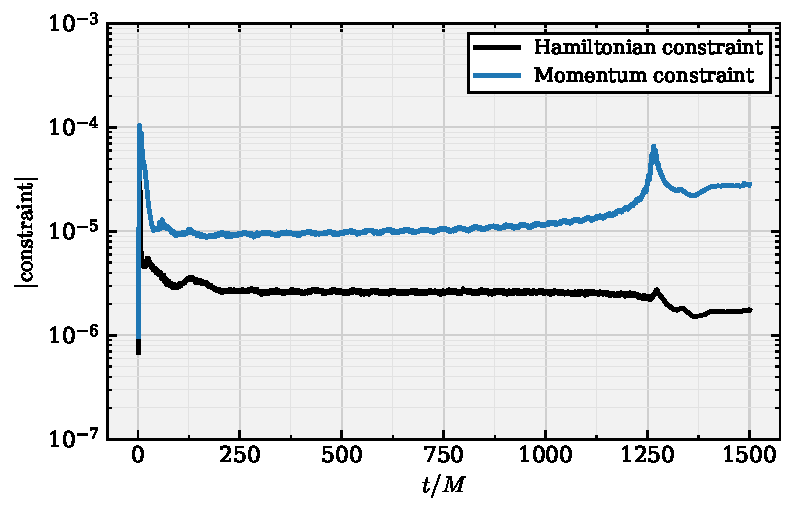
\includegraphics[width=0.65\textwidth]
{Figures/Chapter_2/Constraints/q1/emda_prof_Constraints_Hamiltonian_plus_MomentumSum.pdf}
\caption{
Hamiltonian and combined momentum-constraint violations for a
representative $q=1$ binary evolution. The constraints remain
controlled throughout the inspiral.
}
\label{fig:q1_constraints}
\end{figure}

\begin{figure}[t]
\centering
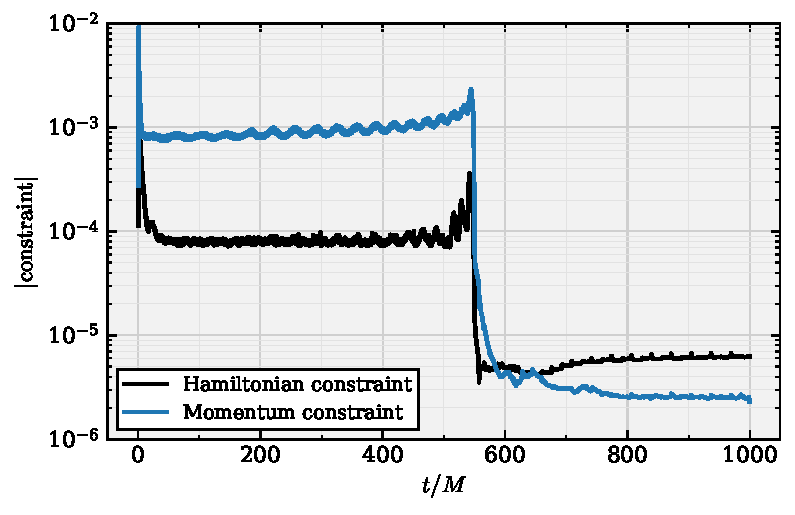
\includegraphics[width=0.65\textwidth]
{Figures/Chapter_2/Constraints/q8/emda_prof_Constraints_Hamiltonian_plus_MomentumSum.pdf}
\caption{
Hamiltonian and combined momentum-constraint violations for the
$q=8$ binary evolution. Although the unequal-mass system places
greater demands on the adaptive mesh, the constraints remain
bounded throughout the simulation.
}
\label{fig:q8_constraints}
\end{figure}

